\section{Additional Mobile Academic Library App Research}
        \subsection{Harvard and Bennett University}
            \paragraph{}
            Harvard and Bennet university had simnular app designs. Harvard's library app, Harvard Library, featured a minimalist home screen with the school logo in the upper-right hand corner, a help button in the lower-left, a 'login' feature in the lower right, and a circular 'start' button in the center. The screen featured only three colors; white, black and crimson red. Clicking the 'start' button pulled up the same login screen that clicking the 'login' button pulled up.  Unfortunately, we were not able to further explore this mobile app because we do not have account affiliated with the University. The home screen for this application can be seen in the following image: 
            \begin{figure}[htbp]
            \centerline{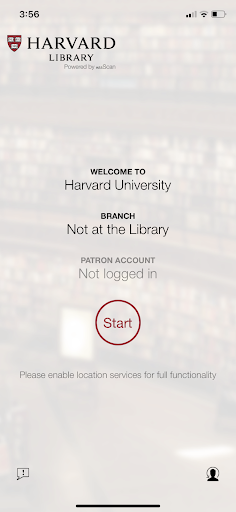
\includegraphics[width=2.5in]{unnamed-4.png}}
            \end{figure}
            The Bennet University app was similar in that unless you had an account, you could not log in and work with it at all. This application had less slick of a design. Some application developers, seem to value exclusivity and privacy. 
        \subsection{Salisbury}
            \paragraph{}
            Sailsbury Universitie's Library app, SU Libraries, featured a noticeably less minimalist design than Harvard's, and had a more unrefined look.  Fortunately, we were able to access the applications features. The home screen included a search bar, and nine features: "Library Hours", "Research Help", "Room Reservations", "Self Checkout", "SU Libraries MakerLab", "Device Availability", "Building Maps", "Helpful Links" and "Contact Information". It also contained a bar at the bottom with five navigation options: "Home", "Library News", "Chat", "My Card" and "About". Additionally, there was a link to the libraries social media accounts. The home screen of this application can be seen in the following image: 
            \begin{figure}[htbp]
            \centerline{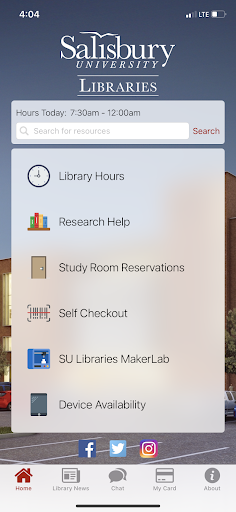
\includegraphics[width=2.5in]{unnamed-3.png}}
            \end{figure}
            \paragraph{}
            The "Library Hours" feature lead to a screen with minimal interactivity. The screen contained the opening and closing times for all days from the current day to approximately three months in advance. The "Research Help" feature took the user to a page with a somewhat similar layout; a page in which you could scroll downward, containing the subjects in which you could get research help. This page, however, was interactive. The user could click on each subject option, taking them to a page with information about who to contact, and how to contact them, if they are seeking research help in that specific area.  The "Study Room Reservations" feature as well as the "Devise Availability" feature has a similar layout to these two.
            \paragraph{}
            The "Building Maps" feature lead to a page containing the layout of each floor of the building. The only interactivity on this page was the option to click on any of the diagrams for an enlarged view of the diagram. 
            \paragraph{}
            The "SU Libraries MakerLab" feature took the user to a page which seemed to function like an app in and of itself. The page it took the user to contained a variety of features relating to the Maker Lab. Such as a feature displaying the time it's open for today as well as a feature displaying which days it is open. It also had a feature taking the user to a page with the Maker Lab policies, a feature allowing users to make an appointment in the maker space, and finally the contact information for the maker space.
        \subsection{University Of Dallas}
            \paragraph{}
            The University of Dallas app had a simple white, black, and Navy blue design. The app consisted of a home screen with four main sections. These sections were "Nearest Libraries", "My Account", "eBooks & eAudio", and "Social". The application also featured a search bar. All of the apps analyzed so far make use of a search functionality. The home screen of this application can be seen in the following image: 
            \begin{figure}[htbp]
            \centerline{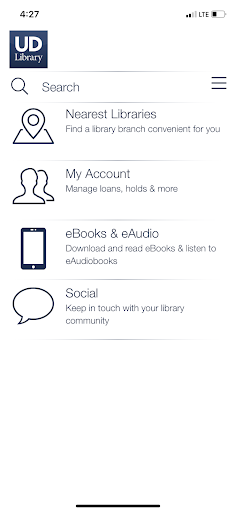
\includegraphics[width=2.5in]{unnamed-2.png}}
            \end{figure}
            \paragraph{}
            \paragraph{}
            Furthermore, like the Harvard app but unlike the Sailsbury app, this app featured a login option. The eBooks & eAudio section linked to a bar code scanner. I think it would be fair to assume this functionality relates to some specific feature at the university of Dallas library. The social tab lead to a link to the libraries social media, namely Facebook, Instagram and Twitter. This seems like a relatively easy functionality to implement, yet still very important. 
        \subsection{University of Sydney}
            \paragraph{}
            This application featured a black white and Orange user interface. The application featured an abundant amount of functions and utilities at the users disposal. These included, but were not limited to: "Libraries", "Book a Study space", "News-Events", "Services", "Scab ISBN" and more. Furthermore, each section had many subsections within it. For example, "Services" encompassed "Study", "Research", "Appointments", and "Disability". They also did indeed contain a section for social media as well as a search bar. The university of Sydney created an extensive application filled with various functionality and features. While the application may seem unwieldy at first, upon familiarizing oneself with the app, it has potential to offer great utility.  
            The home screen of this application can be seen in the following image: 
            \begin{figure}[htbp]
            \centerline{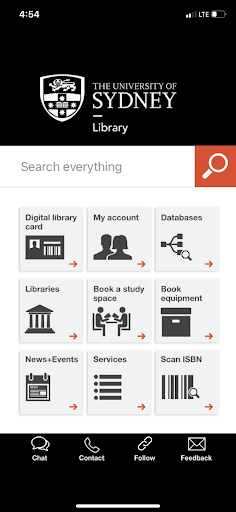
\includegraphics[width=2.5in]{unnamed.png}}
            \end{figure}
            \paragraph{}
        \subsection{Cairn, Parket, Ajman}
            \paragraph{}
            Three other apps which we explored which had a very similar design were that of Cairn University, Parket university, and Ajman University. Each of them had two, potentially three, features. A search with a bar at the top. Presumably, only books could be searched for, but there was also an option to scan books. Below that, two of the apps, Cairn and Parket, featured a scroll bar of book covers at the bottom. These three apps seemed almost identical to one another in style and functionality. 
            
            
        \subsection{Similarities}
        We noticed some similarities among the  applications we analyzed. Firstly, the layout for most of them was the same; a home screen which contained a variety of possible features that, when clicked, would lead to another screen or a pop-up further elaborating on that feature. Some of the specific features were common among many of the applications. For example, four of the eight apps had a functionality for logging in. While this may offer some benefits to the user, it seems difficult to implement and only necessary if you have already implemented some other specific features, such as book checkout. Another feature available in two of the eight apps was a link to the social media; this feature has great utility and would be easy to implement. Finally, there were obvious similarities between the Cairn, Parket, and Ajman apps. They all had the exact same format.
    